\section{Existing implementations}
\label{sect:existing_implementations}

Poengtere at disse implementasjonene er fundamentalt annerledes siden vi jobber
mot sm\aa spro indekser og ikke mot XML-traer o.l som er mer vanlig

\textbf{\underline{\LARGE TODO:}} skrive en del mer om tingene, hvordan de jobber p\aa~ ASTen, om de har relasjonell algebra i det heletatt (exist har vel ikke det?)

\subsection{eXist}
\begin{figure}[h]
  \centering
    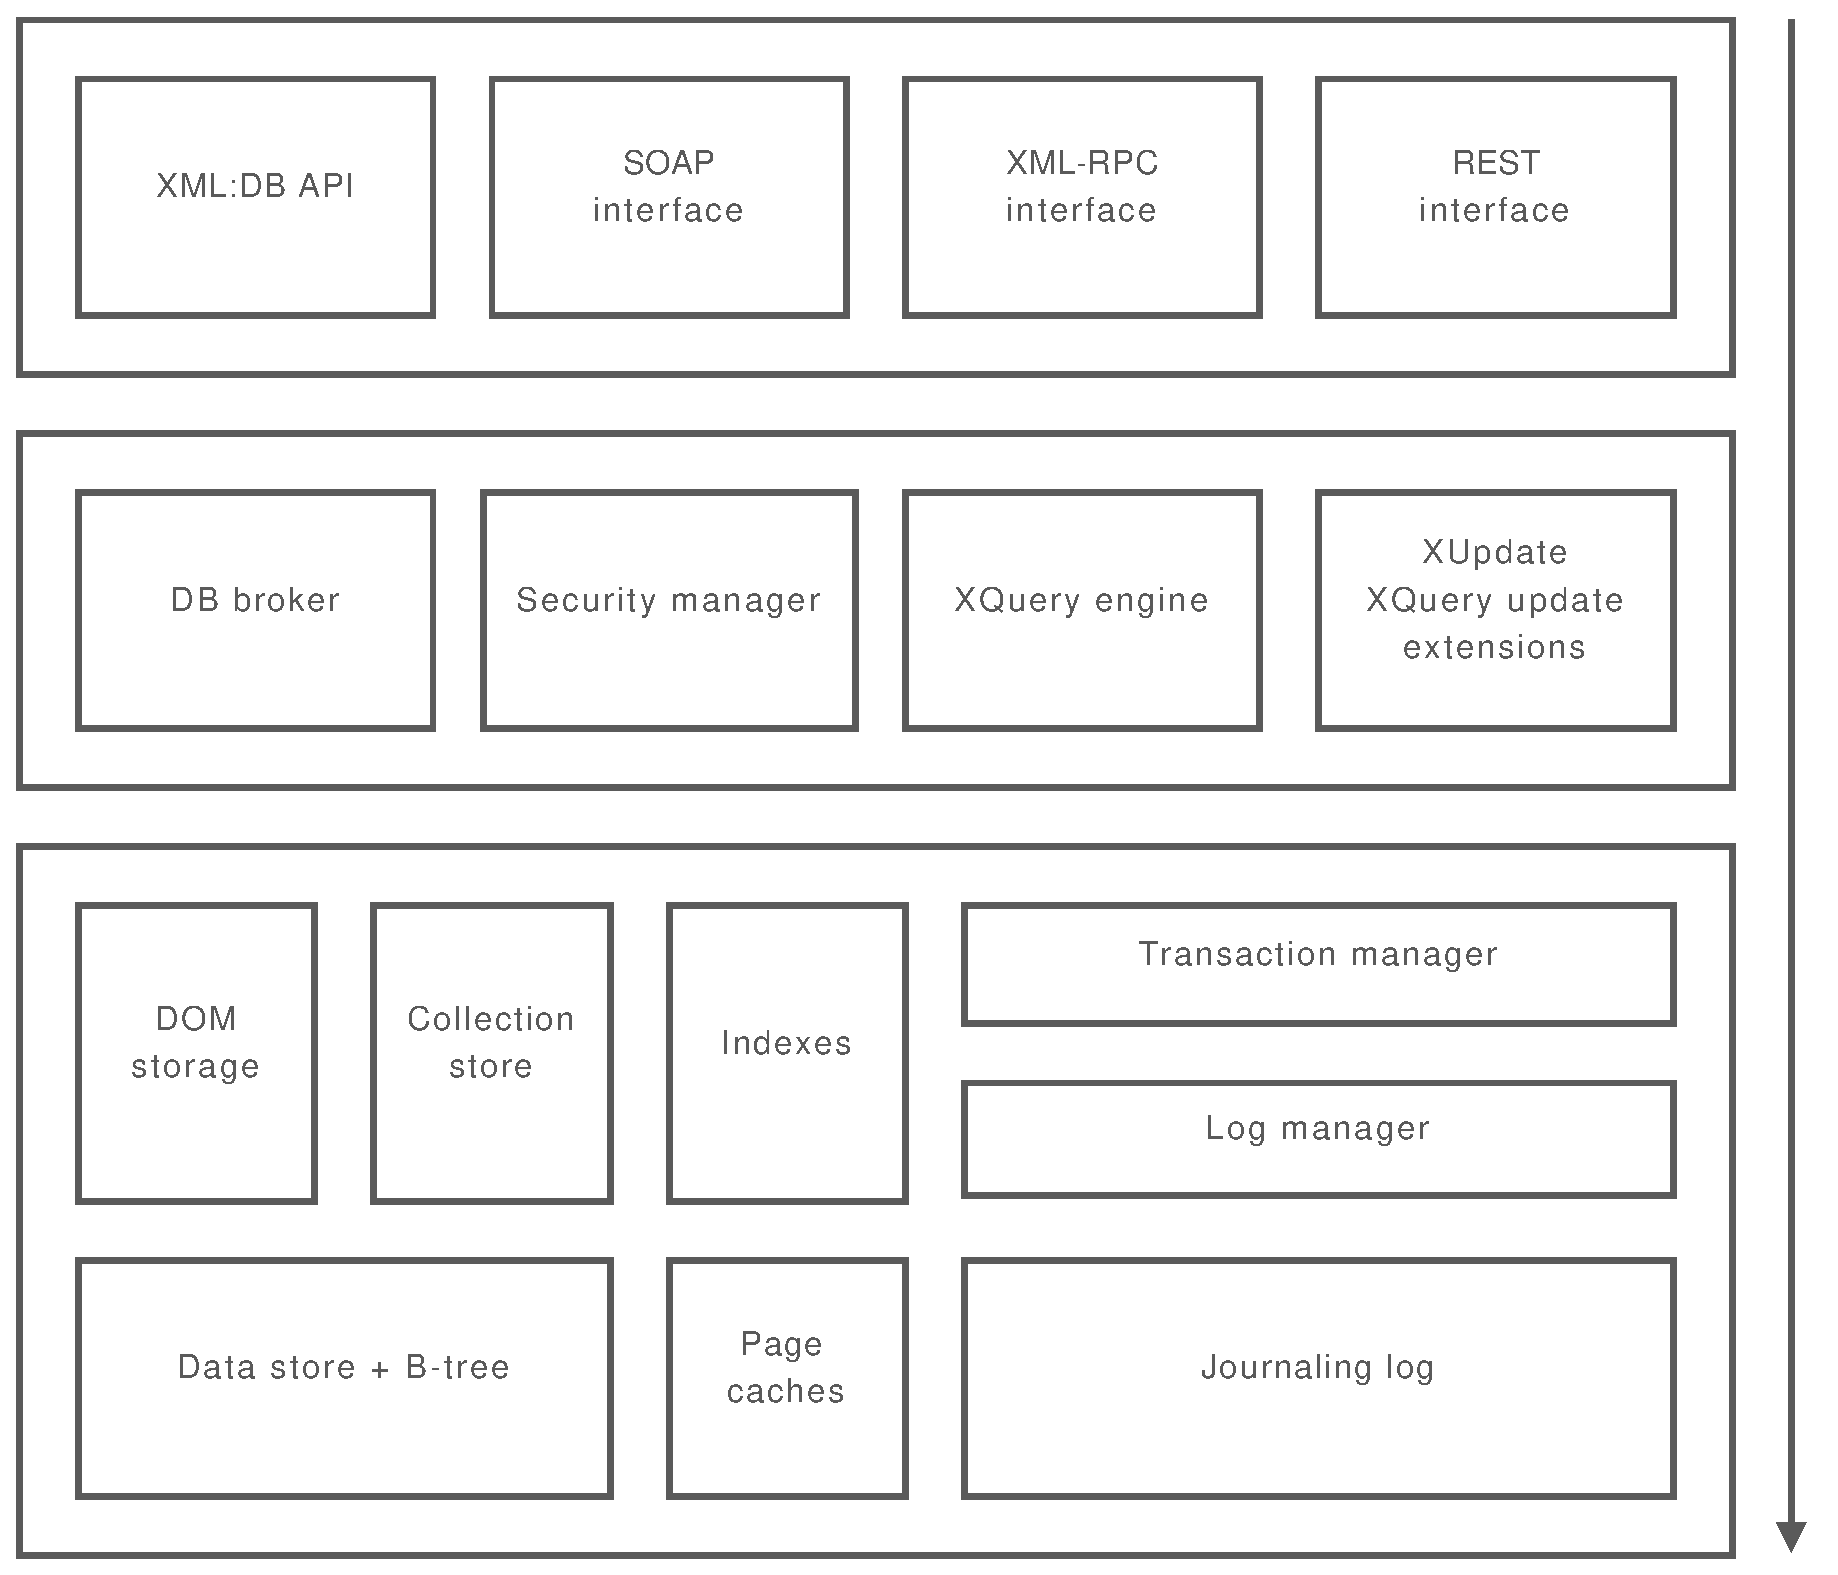
\includegraphics[width=0.9\textwidth]{diagrams/exist_arch}
  \caption[eXist architecture]{eXist architecture, based on architecture sketch
  from \cite{exist_indexdriven}}
\end{figure}
eXist\cite{exist_doc} is an open source native XML database with an XQuery
query processor. The eXist system is written in Java. This system stores native
XML data in B-trees and paged files, and document nodes
in persistent DOM trees\cite{exist_factsheet}. Document collections are stored
in a hierarchical manner similar to a regular file system.

eXist has a numerical indexing scheme for identification of relationships
between nodes (parent/child, ancestor/descendant, previous/next sibling). This
provides a structural index for element attribute nodes. In addition, eXist has
a fulltext index for text and attribute values, and range indexes for typed
values.

Based on these provided index types, the eXist XQuery engine relies on path
join algorithms\cite{exist_idx_drv_query} for efficient computation of node
relationships instead of traditional tree traversals. 

\subsection{Pathfinder}
\label{sect:theory:pathfinder}
\begin{figure}[h]
  \centering
    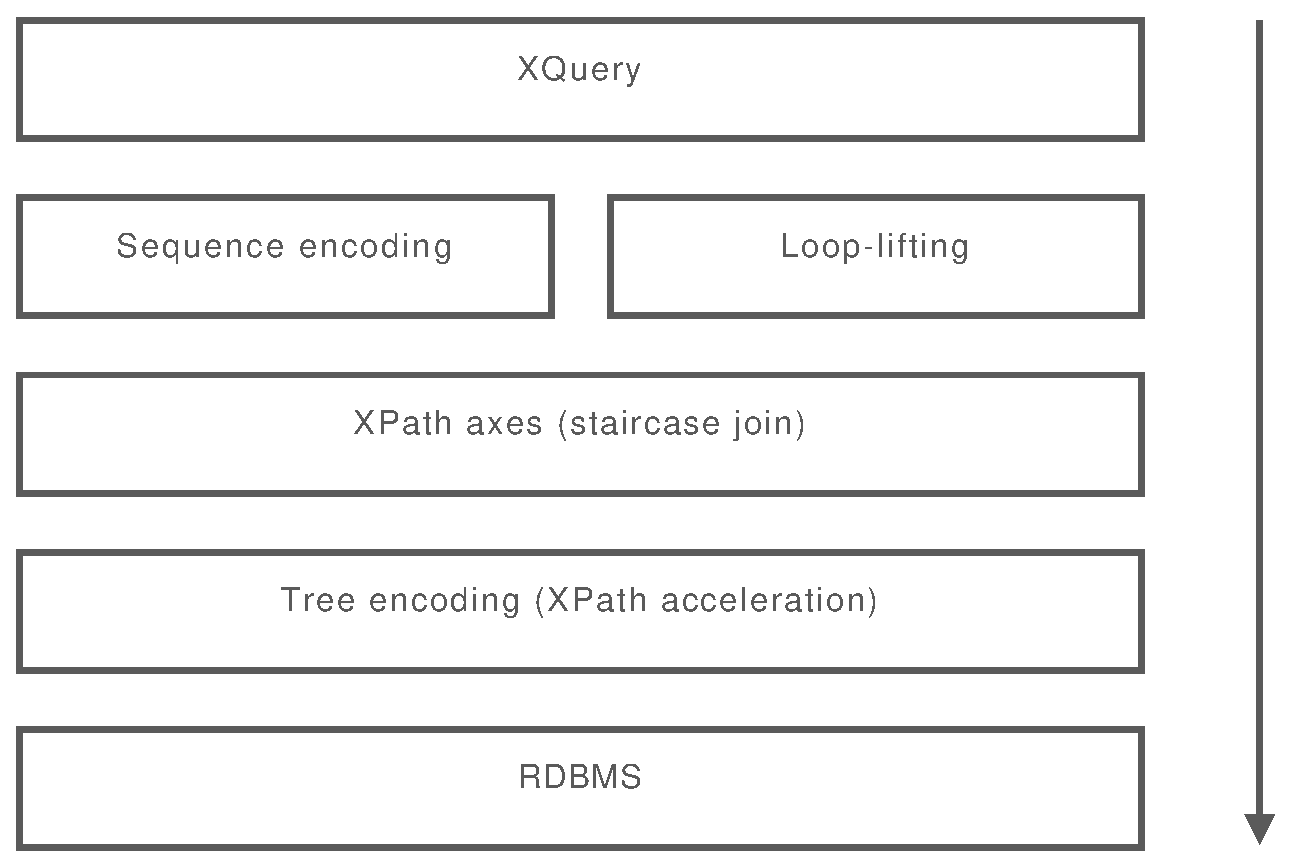
\includegraphics[width=0.6\textwidth]{diagrams/pathfinder_arch}
  \caption{Pathfinder architecture / development stack}
\end{figure}
Pathfinder\cite{pathfinderHome} claims to be a ``purely relational XQuery
processor'', which theoretically can utilize any off-the-shelf RBDMS as a
backend for XQuery execution in a relational context.

The technique for transforming XQuery into relational algebra is called ``loop
lifting''\cite{pathfinder_mothertongue}. Loop lifting is a FLWOR-centric
approach which essentially transforms iterations into joins. Loop lifting is
described in detail in section \ref{sect:trans:loop_lifting}.

As a relational backend, the XQuery processor uses MonetDB, an integrated
component in the Pathfinder project. However, recent versions of Pathfinder is
also capable of producing SQL code for execution on conventional database
systems. As a proof of concept, they performed the XMark test suite on top of
the IBM DB2 system\cite{pathfinder_sql}.

\subsection{Galatex}
\begin{figure}[h]
  \centering
    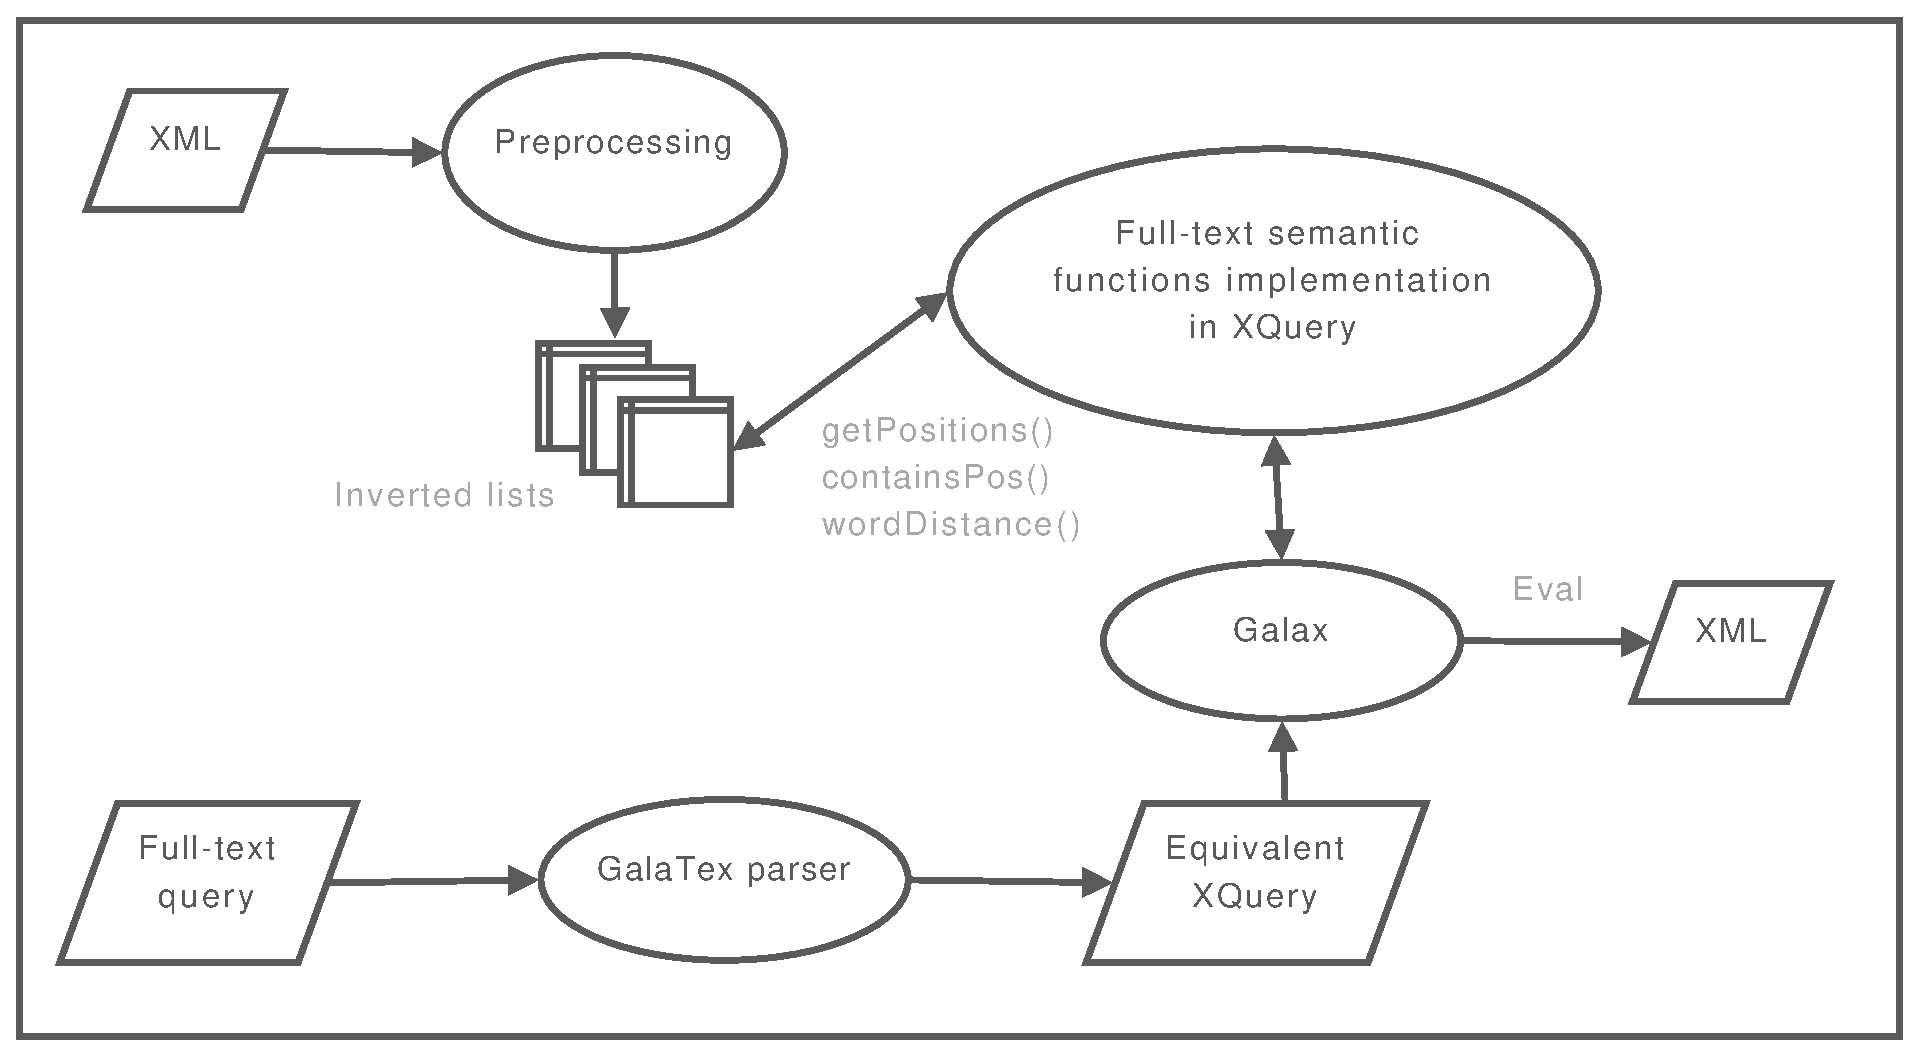
\includegraphics[width=1\textwidth]{diagrams/galatex_arch}
  \caption[GalaTex architecture]{Galatex architecture, based on architecture described on
  the GalaTex website\cite{galatex}}
  \label{figure:galatex:arch}
\end{figure}
Galatex is claimed to be the first full implementation of the W3C XQuery 1.0 
and XPath 2.0 Full-Text 1.0 specification\cite{w3c01}. As can be seen in figure
\ref{figure:galatex:arch}, Galatex translates the full-text parts of the query
into standard normalized XQuery (XQuery Core\cite{xquery_semantics}, also
described in section \ref{sect:theory:xquery:XQcore}) in the Galatex parser. The equivalent
XQuery query is then executed on the Galax query processor.

The most interesting aspect of Galatex is its full-text capabilities. This is
realized first and foremost by an implementation of the AllMatches data model
proposed by W3C\cite{w3c01}. Additionally, as mentioned above, the full-text fragments of the queries are
translanted into corresponding functions in regular XQuery. 

\subsection{Trait comparison matrix}
\label{sect:theory:existing_implementations:comparison}
This section will compare some important traits of the described
implementations, and will outline their implications.
\begin{figure}[!h]
	\centering
	\begin{tabular}{ | p{3cm} | c | c | c |}
	\hline
	& eXist & Pathfinder & GalaTex \\ \hline
	Normalization to XQuery Core & Yes & Yes & Yes \\ \hline
	Relational backend & No & Yes & No \\ \hline
	Full-text extensions & No & No & Yes \\ \hline
	Test suite coverage & 99.4\% & 99.4\% & n/a \\ \hline
	Free source code & Yes & Yes & Yes  \\
	\hline
	\end{tabular}
	\caption{Comparison of implementation traits}
	\label{figure:comparison_matrix}
\end{figure}
The traits chosen for the comparison matrix in figure
\ref{figure:comparison_matrix} are chosen due to their relevance to this
project. As can be seen, there is a spread in diversity across these
implementations. In particular, Pathfinder is the only implementation with a
relational backend.